\documentclass[conference]{IEEEtran}
\makeatletter
\def\ps@headings{%
\def\@oddhead{\mbox{}\scriptsize\rightmark \hfil \thepage}%
\def\@evenhead{\scriptsize\thepage \hfil \leftmark\mbox{}}%
\def\@oddfoot{}%
\def\@evenfoot{}}
\makeatother
\pagestyle{headings}

\hyphenation{op-tical net-works semi-conduc-tor}


\usepackage{subfigure}
\usepackage{soul}

\usepackage{algorithmic}
\usepackage[ruled,vlined]{algorithm2e}

\ifCLASSINFOpdf
  \usepackage[pdftex]{graphicx}
  % declare the path(s) where your graphic files are
  % \graphicspath{{../pdf/}{../jpeg/}}
  % and their extensions so you won't have to specify these with
  % every instance of \includegraphics
  % \DeclareGraphicsExtensions{.pdf,.jpeg,.png}
\else
  % or other class option (dvipsone, dvipdf, if not using dvips). graphicx
  % will default to the driver specified in the system graphics.cfg if no
  % driver is specified.
  % \usepackage[dvips]{graphicx}
  % declare the path(s) where your graphic files are
  % \graphicspath{{../eps/}}
  % and their extensions so you won't have to specify these with
  % every instance of \includegraphics
  % \DeclareGraphicsExtensions{.eps}
\fi
% graphicx was written by David Carlisle and Sebastian Rahtz. It is
% required if you want graphics, photos, etc. graphicx.sty is already
% installed on most LaTeX systems. The latest version and documentation can
% be obtained at:
% http://www.ctan.org/tex-archive/macros/latex/required/graphics/
% Another good source of documentation is "Using Imported Graphics in
% LaTeX2e" by Keith Reckdahl which can be found as epslatex.ps or
% epslatex.pdf at: http://www.ctan.org/tex-archive/info/
%
% latex, and pdflatex in dvi mode, support graphics in encapsulated
% postscript (.eps) format. pdflatex in pdf mode supports graphics
% in .pdf, .jpeg, .png and .mps (metapost) formats. Users should ensure
% that all non-photo figures use a vector format (.eps, .pdf, .mps) and
% not a bitmapped formats (.jpeg, .png). IEEE frowns on bitmapped formats
% which can result in "jaggedy"/blurry rendering of lines and letters as
% well as large increases in file sizes.
%
% You can find documentation about the pdfTeX application at:
% http://www.tug.org/applications/pdftex

\begin{document}
\title{Titolo del progetto svolto}

% Author names 
% note positions of commas and nonbreaking spaces ( ~ ) LaTeX will not break
% a structure at a ~ so this keeps an author's name from being broken across
% two lines.
% use \thanks{} to gain access to the first footnote area
% a separate \thanks must be used for each paragraph as LaTeX2e's \thanks
% was not built to handle multiple paragraphs
\author{
Nome Autore1\IEEEauthorrefmark{1},
Nome Autore2\IEEEauthorrefmark{1},
\\
\IEEEauthorblockA{\IEEEauthorrefmark{1} DISI, University of Bologna, Italy \\
 \\
Emails: autore1@email.it, autore2@email.it, autore3@email.it}}




% make the title area
\maketitle

% The Abstract
\begin{abstract}
Riassumi qui il succo del progetto, in 20-30 righe.

\end{abstract}



\section{Introduction}
Descrivi qui il contesto generale, i contributi del progetto, e la struttura del documento.
 

\section{Related works}
Fornisci una breve rassegna di articoli di ricerca, software, prototipi o tecnologie che sono collegate in qualche modo al problema affrontato nel progetto. Tutti i lavori devono essere referenziati ed inseriti nella Bibliografia.

\section{Architecture}
Il sistema \'e stato sviluppato in modo da poter girare su dispositivi Android, lasciando in questo modo la possibilità di essere utilizzato in larga scala e senza costi aggiuntivi al prezzo del dispositivo stesso.
Suddetto applicativo è costituito da due tipologie di layer applicativi che potremmo denominare Publisher e Observer così da poter rendere il pi\'u intuitivo possibile il ruolo da loro ricoperto.
\begin{figure}[h!]
	\centering
	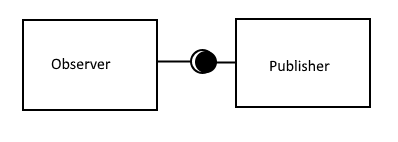
\includegraphics[width=0.7\linewidth]{ps}
	\caption[Concetti base]{}
	\caption{}
	\label{fig:ps}
\end{figure}
Il ruolo del Publisher viene assunto da tutti i dispositivi in possesso ai pedoni. Il loro compito principale \'e quello di avvisare i veicoli circostanti riguardo la propria posizione corrente.
Tutti i veicoli presenti sulla strada, invece, sono Observer ed hanno l'obbligo di ascoltare in ogni istante i Publisher, elaborare i loro dati ed avvertire il conducente.
La struttra della rete risulta dunque essere un miscuglio approsimatamente omogeneo di Publisher ed Observer.
\begin{figure}[h!]
	\centering
	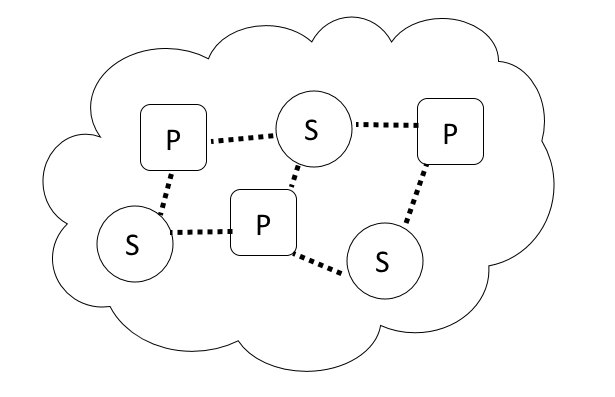
\includegraphics[width=0.7\linewidth]{net}
	\caption[Rete]{}
	\caption{}
	\label{fig:net}
\end{figure}
La forza di questo sistema è il fatto che la rete non preveda una vera e propria sturuttra, ma che si adatti a quelle che sono le limitazioni dell'ambiente circostante.
Questa qualità del sistema lo rende flessibile e particolarmente scalabile.

\section{Implementation}
Descrivi come e\' stato implementato il sistema, ossia tecnologie utilizzate, linguaggi, APIs, etc. Nel caso, fornisci pseudo-codice degli algoritmi
piu\' interessanti sviluppati nel progetto.

- Ambiente
- IDE
- Test effettuati (BLUETOOTH)
- WiFi Direct (Problemi riscontrati ed implementazione in android)
- Modello di Localizzazione (Low Energy)
- Modello di Previsione

\section{Performance evaluation}
Illustra qui i risultati sperimentali (simulazioni o esperimenti) che catturano le prestazioni del sistema realizzato. Chiarisci quali sono gli indici di stima
e come sono calcolati. Inserisci un breve commento per ogni grafico.

\section{Conclusioni}
Conclusioni, possibili sviluppi futuri e limitazioni del progetto realizzato

%% Inserisci bibliografia dei lavori citati (consiglio l'utilizzo di bibtex)
\bibliographystyle{plain}
\begin{thebibliography}{15}

\bibitem{NomeRiferimento}
\newblock{Lista Autori} 
\newblock{Titolo Lavoro}
\newblock{\textit{Nome Rivista o Convegno}}, pagine, anno pubblicazione.

\end{thebibliography}
\end{document}